\section{遷移問題への拡張}\label{chap:trans}

\subsection{遷移問題の概要}

根付き全域森の遷移問題への拡張について,新たに
\textbf{初期状態}と\textbf{目的状態}を定義する.初期状態と
目的状態は,それぞれ対象となるグラフの根付き全域森の実行
可能解である.

根付き全域森の遷移問題は,入力として初期状態と目的状態が
与えられ,各状態で根付き全域森の制約を満たしながら,
状態が遷移する際に変化する辺の数は$d$個以下である.という
\textbf{遷移制約}を新たに設定する.

図\ref{fig:trans}は,遷移制約を$d=2$とした場合での遷移問題の例である.

\begin{figure*}[ht]
 \begin{center}
  \begin{tabular}{cc}
   \subfigure[$t=0$ (初期状態)]{
   %%%%%%%%%%%%%%%%%%%%%%%%%%%%%%%%%%%%%%%%%%%%%%%%%%
% 実行例(t=0) (第6章で使う)
%%%%%%%%%%%%%%%%%%%%%%%%%%%%%%%%%%%%%%%%%%%%%%%%%%

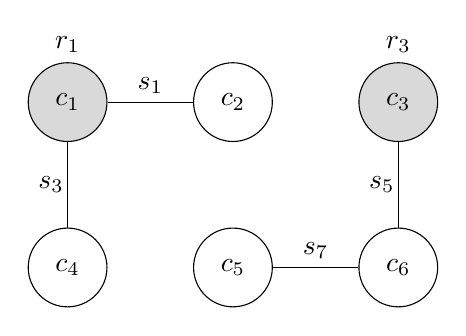
\begin{tikzpicture}[x=1.5cm,y=1.5cm,scale=0.7]

 % 設定
 \tikzset{root/.style={circle,draw=black,fill=gray!30,minimum size=1cm}}
 \tikzset{node/.style={circle,draw=black,minimum size=1cm}}
 
 % 補助線
 % \draw [help lines,blue,step=2cm] (-3,0) grid (3,-3);

 % 時間 %
 % \node[rectangle,draw=black] at (-3,1) {$t=0$};

 % root %
 \node[root] at (-2,0) (1){$c_1$};
 \node[above=0.5cm] at (1) {$r_1$};
 \node[root] at (2,0) (3){$c_3$};
 \node[above=0.5cm] at (3) {$r_3$};

 % node %
 \node[node] at (0,0) (2){$c_2$};
 \node[node] at (-2,-2) (4){$c_4$};
 \node[node] at (0,-2) (5){$c_5$};
 \node[node] at (2,-2) (6){$c_6$};

 % 繋がっていない辺は破線
 %\foreach \u / \v in {2/3, 2/5, 4/5}
 %\draw [dashed] (\u) -- (\v);
 % 繋がってる辺は実線
 \foreach \u / \v in {1/2, 1/4, 3/6, 5/6}
 \draw (\u) -- (\v);

 % スイッチ switch %
  \node at (-1,0.2) {$s_1$};
 % \node at (1,0.2) {$s_2$};
  \node at (-2.2,-1) {$s_3$};
 % \node at (-0.2,-1) {$s_4$};
  \node at (1.8,-1) {$s_5$};
 % \node at (-1,-1.8) {$s_6$};
  \node at (1,-1.8) {$s_7$};
 %

\end{tikzpicture}

%%%%%%%%%%%%%%%%%%%%%%%%%%%%%%%%%%%%%%%%%%%%%%%%%%%%%%%%%%
%%% Local Variables:
%%% mode: japanese-latex
%%% TeX-master: paper.tex
%%% End:

   \label{trans-1} \hspace{1cm}
   } &
	   \subfigure[$t=1$]{
	   %%%%%%%%%%%%%%%%%%%%%%%%%%%%%%%%%%%%%%%%%%%%%%%%%%
% 実行例(t=1) (第6章で使う)
%%%%%%%%%%%%%%%%%%%%%%%%%%%%%%%%%%%%%%%%%%%%%%%%%%

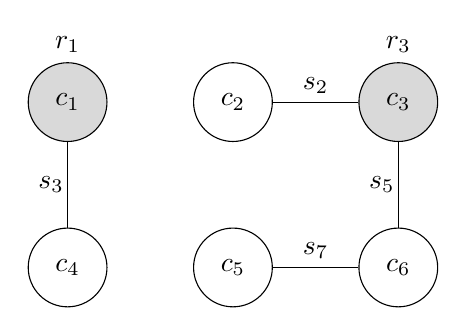
\begin{tikzpicture}[x=1.5cm,y=1.5cm,scale=0.7]

 % 設定
 \tikzset{root/.style={circle,draw=black,fill=gray!30,minimum size=1cm}}
 \tikzset{node/.style={circle,draw=black,minimum size=1cm}}
 
 % 補助線
 % \draw [help lines,blue,step=2cm] (-3,0) grid (3,-3);

 % 時間 %
 % \node[rectangle,draw=black] at (-3,1) {$t=1$};

 % root %
 \node[root] at (-2,0) (1){$c_1$};
 \node[above=0.5cm] at (1) {$r_1$};
 \node[root] at (2,0) (3){$c_3$};
 \node[above=0.5cm] at (3) {$r_3$};

 % node %
 \node[node] at (0,0) (2){$c_2$};
 \node[node] at (-2,-2) (4){$c_4$};
 \node[node] at (0,-2) (5){$c_5$};
 \node[node] at (2,-2) (6){$c_6$};

 % 繋がっていない辺は破線
 %\foreach \u / \v in {2/3, 2/5, 4/5}
 %\draw [dashed] (\u) -- (\v);
 % 繋がってる辺は実線
 \foreach \u / \v in {2/3, 1/4, 3/6, 5/6}
 \draw (\u) -- (\v);

 % スイッチ switch %
 % \node at (-1,0.2) {$s_1$};
 %
 \node at (1,0.2) {$s_2$};
 \node at (-2.2,-1) {$s_3$};
 % \node at (-0.2,-1) {$s_4$};
 \node at (1.8,-1) {$s_5$};
 % \node at (-1,-1.8) {$s_6$};
 \node at (1,-1.8) {$s_7$};
 %

\end{tikzpicture}

%%%%%%%%%%%%%%%%%%%%%%%%%%%%%%%%%%%%%%%%%%%%%%%%%%%%%%%%%%
%%% Local Variables:
%%% mode: japanese-latex
%%% TeX-master: paper.tex
%%% End:
 
	   \label{trans-2}   
	   } \\ \vspace{0.3cm}
   \subfigure[$t=3$ (目的状態)]{
   %%%%%%%%%%%%%%%%%%%%%%%%%%%%%%%%%%%%%%%%%%%%%%%%%%
% 実行例(t=3) (第6章で使う)
%%%%%%%%%%%%%%%%%%%%%%%%%%%%%%%%%%%%%%%%%%%%%%%%%%
\begin{tikzpicture}[scale=0.6]

 % 設定
 \tikzset{node/.style={circle,draw=black,fill=white}}

 \definecolor{edge1}{RGB}{191,0,0}
 \definecolor{node1}{RGB}{249,200,200}
 \definecolor{edge3}{RGB}{38,38,134}
 \definecolor{node3}{RGB}{200,200,249}

 % 補助線
 % \draw [help lines,blue] (0,0) grid (20,6);

 % node %
 \node[circle, ultra thick, draw=edge1, fill=node1](out1){1};
 \node[node, fill=node3, right=of out1] (out2){2};
 \node[circle, ultra thick, draw=edge3,fill=node3, right=of out2](out3){3};
 \node[node, fill=node3, below=of out1] (out4){4};
 \node[node, fill=node3, below=of out2] (out5){5};
 \node[node, fill=node3, below=of out3] (out6){6};

 \foreach \u / \v in {}
 \draw [very thick, edge1] (\u) -- (\v);

 \foreach \u / \v in {out2/out3,out2/out5,out4/out5,out5/out6}
 \draw [very thick, edge3](\u) -- (\v);
\end{tikzpicture}

%%%%%%%%%%%%%%%%%%%%%%%%%%%%%%%%%%%%%%%%%%%%%%%%%%%%%%%%%%
%%% Local Variables:
%%% mode: japanese-latex
%%% TeX-master: paper.tex
%%% End:

   \label{trans-4}  \hspace{1cm} 
   } &
	   \subfigure[$t=2$]{
	   %%%%%%%%%%%%%%%%%%%%%%%%%%%%%%%%%%%%%%%%%%%%%%%%%%
% 実行例(t=2) (第6章で使う)
%%%%%%%%%%%%%%%%%%%%%%%%%%%%%%%%%%%%%%%%%%%%%%%%%%

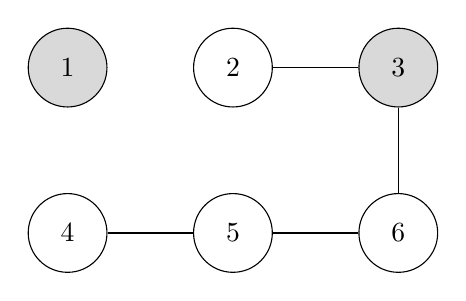
\begin{tikzpicture}[x=1.5cm,y=1.5cm,scale=0.7]

 % 設定
 \tikzset{root/.style={circle,draw=black,fill=gray!30,minimum size=1cm}}
 \tikzset{node/.style={circle,draw=black,minimum size=1cm}}
 
 % 補助線
 % \draw [help lines,blue,step=2cm] (-3,0) grid (3,-3);

 % 時間 %
 % \node[rectangle,draw=black] at (-3,1) {$t=2$};

 % root %
 \node[root] at (-2,0) (1){$1$};
% \node[above=0.5cm] at (1) {$r_1$};
 \node[root] at (2,0) (3){$3$};
 %\node[above=0.5cm] at (3) {$r_3$};

 % node %
 \node[node] at (0,0) (2){$2$};
 \node[node] at (-2,-2) (4){$4$};
 \node[node] at (0,-2) (5){$5$};
 \node[node] at (2,-2) (6){$6$};

 % 繋がっていない辺は破線
 %\foreach \u / \v in {2/3, 2/5, 4/5}
 %\draw [dashed] (\u) -- (\v);
 % 繋がってる辺は実線
 \foreach \u / \v in {2/3, 4/5, 3/6, 5/6}
 \draw (\u) -- (\v);

 % スイッチ switch %
 % \node at (-1,0.2) {$s_1$};
 % \node at (1,0.2) {$s_2$};
 % \node at (-2.2,-1) {$s_3$};
 % \node at (-0.2,-1) {$s_4$};
 % \node at (1.8,-1) {$s_5$};
 % \node at (-1,-1.8) {$s_6$};
 % \node at (1,-1.8) {$s_7$};
 %

\end{tikzpicture}

%%%%%%%%%%%%%%%%%%%%%%%%%%%%%%%%%%%%%%%%%%%%%%%%%%%%%%%%%%
%%% Local Variables:
%%% mode: japanese-latex
%%% TeX-master: paper.tex
%%% End:

	   \label{trans-3}
	   } \\
  \end{tabular}
  \caption{遷移問題の例}
  \label{fig:trans}
 \end{center}
\end{figure*}

\subsection{ASP符号化}
今回考案した符号化は,外部プログラムによるループを用いた
インクリメンタル探索を行うものと,ASPソルバー{\clingo}の
インクリメンタル探索ライブラリを使用した2種類の符号化である.

外部プログラムを用いる符号化をコード\ref{code:roop}に示す.
遷移問題への拡張について基本的には,コード\ref{code:srf2.lp}に
出現する各アトムに,状態数を表す引数\code{T}を追加する.これ
により各状態\code{T}における根付き全域森を探索する.1行目の
\code{t(0..t)}は,0から$t$までの各状態数を定義している.なお,
$t$は外部プログラムによって与えられる変数($t \geq 0$)である.
この状態数を増やして解が得られるまで実行することでインクリ
メンタル探索を行う.

4行目のルールは,初期条件として,与えられる初期状態と状態0における
根付き全域森が一致することを表す制約である.\code{init_Forest(X,Y)}
は初期状態での根付き全域森に含まれる辺を表す.同様に7行目のルールで,
終了条件として,与えられる目的状態と状態$t$における根付き全域森が一致
することを表す.\code{goal_Forest(X,Y)}は目的状態での根付き全域森に含ま
れる辺を表す.10〜21行目までは,先に述べたように根付き全域森の各制約に
状態数\code{T}を追加したルールである.

24行目から26行目までは,遷移制約を表すルールであり,24,25行目は,
状態\code{T-1}で森に含まれていない辺が状態\code{T}で森に含まれる
辺となった場合,あるいはその逆を\code{dist(X,Y,T)}として生成する.
26行目で各状態\code{T}について変化した辺の数である\code{dist(X,Y,T)}
の数が$d$以下であることを一貫性制約で表している.

次に,ライブラリを用いたインクリメンタル探索を行う符号化をコード
\ref{code:incmode}に示す.

1行目はSATが出力されるまで求解を行うことを表し,2行目は$t=0$から
探索を行うことを示している.ライブラリを用いるASPのコードは,
\code{base}部分,\code{step}部分,\code{check}部分に分けられる.

\code{base}部分は,最初の1回目の探索時にのみ符号化を行うルールであり,
ここでは初期条件を9行目に記述している.

15〜34行目の\code{step}部分は,各状態において満たすべきルールを記述する
部分であり,探索回数を増やす毎にこの部分の符号化が追加される.ここでは
根付き全域森の制約と遷移制約を記述している.

最後に,\code{check}部分では終了条件を記述しており,ある状態$t$で
このルールが成り立つとき,そこで探索を終えることを意味している.

ライブラリを用いることで,ソルバーを起動する毎に発生するオーバヘッドの
減少や,前に実行した探索で得られた学習節を利用することができるので,
外部プログラムによって繰り返し探索するよりも,高速に解が得られると考えられる.

\onecolumn

%%%%%%%%%%%%%%%%%%%%%%%%%%%%%%%%%
\lstinputlisting[float=h,caption={%
外部プログラムを用いるASP符号化},%
captionpos=b,frame=single,label=code:roop,%
numbers=left,%
breaklines=true,%
columns=fullflexible,keepspaces=true,%
basicstyle=\ttfamily\scriptsize]{code/trans-const.lp}
%%%%%%%%%%%%%%%%%%%%%%%%%%%%%%%%%
%%%%%%%%%%%%%%%%%%%%%%%%%%%%%%%%%
\lstinputlisting[float=h,caption={%
ライブラリを用いるASP符号化},%
captionpos=b,frame=single,label=code:incmode,%
numbers=left,%
breaklines=true,%
columns=fullflexible,keepspaces=true,%
basicstyle=\ttfamily\scriptsize]{code/dnet-trans.lp}
%%%%%%%%%%%%%%%%%%%%%%%%%%%%%%%%% 
\twocolumn